\subsection{Additional learning comparisons}\label{app:legacy-learning}\label{app:learning-protocol}\label{app:calibration-protocol}
The attribution-column error of a learned model splits exactly into a
weight-shift and a response term ($L$/$S$: learned/direct in
Eq.~\eqref{eq:Cdef}):
\begin{equation}
c_j^{L}-c_j^{S}
=\Delta q_j\int_0^1(D_\lambda^{L}-D_\lambda^{S})J_j^{S}\,\mathrm{d}\lambda
+\Delta q_j\int_0^1D_\lambda^{L}(J_j^{L}-J_j^{S})\,\mathrm{d}\lambda,
\label{eq:coldecomp}
\end{equation}
satisfied entrywise within $10^{-10}$ TSTT units on the 96 test paths;
the weight-shift term has querywise median norm at most 0.2\% of the
reference column and the response term is larger in every seed--query
unit.

\paragraph{Six objectives under a fair weight search.}
Table~\ref{tab:fairmethods} completes the objective comparison under
the shared continuation budget and the common validation-only weight
search (Appendix~\ref{app:pairs-v102}). Each objective's auxiliary
term is normalized by a scale carrying that objective's own units ---
in particular the weighted-response term by its reference scale
$v_j^2=\langle\|D^SJ_j^S\|_2^2\rangle_j$ rather than the unweighted
scale --- so that a common weight grid explores comparable
regularization ranges; under this normalization every objective trains
at a properly selected weight. Weighted-response supervision reaches a
column error of $15.21\%$ at its selected weight, improves 84 of 96
paths, and trains across the whole low-to-mid weight range; the
unweighted form is the simplest member of the family and attains the
lowest errors on every metric. With validation-selected weights, both
endpoint objectives improve attribution accuracy relative to flow-only
training ($21.18\%\to16.2\%$ in column error), although their errors
remain above those of the response-supervised objectives. The
boundary-seminorm objective shows the largest validation--test gap:
its validation boundary error decreases monotonically with the weight
up to the selected $\lambda^*=0.3$ and reaches the lowest validation
value of any objective, yet its test column error at that weight stays
above flow-only training ($24.18\%$, improved on only 8 of 96 paths).
As Section~\ref{sec:pairresults} discusses through the seminorm
kernel, optimizing the boundary value alone does not repair the
underlying response field, whereas supervising that field improves
every spatial error metric.
\begin{table}[t]\centering\footnotesize
\caption{Six supervision objectives on the same 96 test demand paths,
each at its validation-selected weight $\lambda^*$ under the shared
continuation budget and uniform selection rule
(Appendix~\ref{app:pairs-v102}); the weighted-response objective is
normalized by its own reference scale $v_j$. Entries are medians of
path-level values; improved: paths on which the objective lowers the
column (family-boundary) error relative to flow-only
training.}\label{tab:fairmethods}
\setlength{\tabcolsep}{5pt}
\begin{tabular*}{\tblwidth}{@{\extracolsep{\fill}}lcccc cc}
\toprule
Objective & $\lambda^*$ & Flow pred.\ (\%) & Column (\%) & Family boundary (\%) & \multicolumn{2}{c}{Improved vs.\ flow}\\
\cmidrule(lr){6-7}
& & & & & col. & fam.\\
\midrule
Flow only & --- & 0.032 & 21.18 & 8.74 & --- & ---\\
Response supervision & 1 & 0.029 & 14.19 & 5.75 & 92/96 & 90/96\\
Weighted response & 0.1 & 0.032 & 15.21 & 6.93 & 84/96 & 79/96\\
Boundary seminorm & 0.3 & 0.037 & 24.18 & 7.21 & 8/96 & 45/96\\
Endpoint-edge & 0.3 & 0.035 & 16.23 & 7.46 & 72/96 & 66/96\\
\quad + cut term$^{\dag}$ & 0.3 & 0.035 & 16.26 & 7.47 & 72/96 & 67/96\\
\bottomrule\end{tabular*}\end{table}
\noindent$^{\dag}$The endpoint-cut bundle is the endpoint-edge
objective plus a boundary term at a fixed ratio of $0.01$; it is
reported as an ablation of that fixed mixture ratio, not as an
independently tuned competitor.
\begin{figure}[t]
\centering
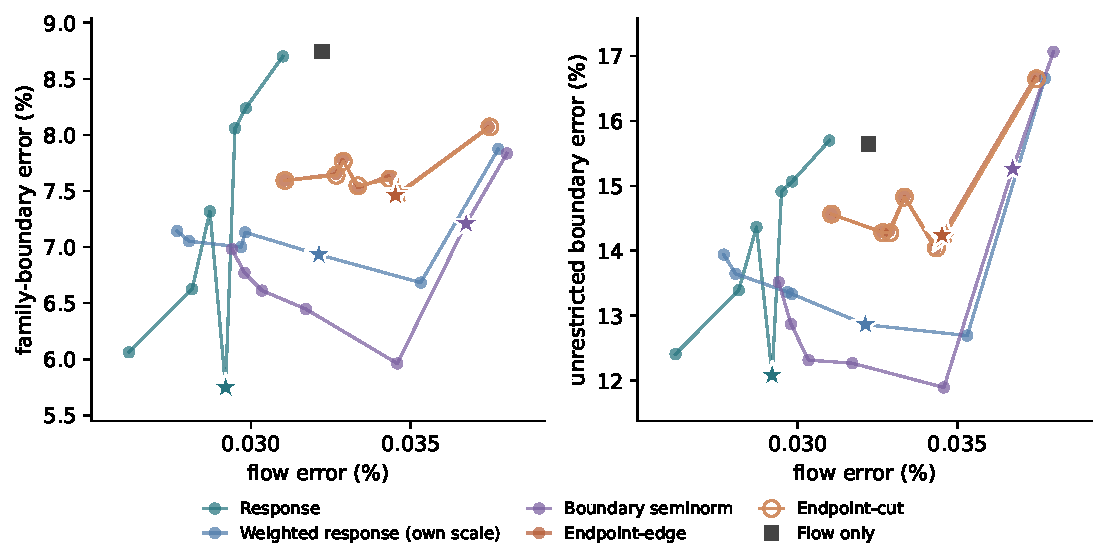
\includegraphics[width=\linewidth]{../figures/fig_v110_pareto.pdf}
\caption{Explanation--flow trade-off of the six supervision objectives
across the weight grid, on the 96 Sioux Falls test paths. Each point
is one (objective, weight) configuration: median flow error against
median family-boundary error (left) and unrestricted boundary error
(right); the validation-selected weight of each objective is starred.
Response supervision sweeps the efficient frontier in both panels,
interpolating between flow-only behavior and the lowest boundary
error. Under its own scale normalization the weighted-response
objective tracks the same band across the low-to-mid weights; only the
largest weight violates the validation flow-accuracy constraint and
selects the initial checkpoint. The boundary-seminorm objective
reaches its best errors only at unselected intermediate weights, and
the endpoint objectives (nearly coincident; the cut term is a
fixed-ratio minor addition) trace interior curves.}
\label{fig:v109pareto}
\end{figure}

\subsection{Group-level uncertainty for the 96-path comparison}\label{supp:learningdetail}
\begin{table}[pos=htbp]\centering\footnotesize
\caption{Per-seed medians of path-level values on the 96 paths and
path-level improvement counts (response vs.\ flow supervision).}\label{tab:fiveseed}
\setlength{\tabcolsep}{4.5pt}
\begin{tabular*}{\tblwidth}{@{\extracolsep{\fill}}r cc cc cc}
\toprule
& \multicolumn{2}{c}{Column (\%)} & \multicolumn{2}{c}{Geometric (\%)} & \multicolumn{2}{c}{Improved paths}\\
\cmidrule(lr){2-3}\cmidrule(lr){4-5}\cmidrule(lr){6-7}
Seed & flow & resp. & flow & resp. & col. & geo.\\
\midrule
0 & 19.55 & 15.93 & 8.40 & 5.67 & 85/96 & 84/96\\
1 & 15.66 & 12.44 & 7.07 & 4.57 & 80/96 & 84/96\\
2 & 22.81 & 14.91 & 9.08 & 6.52 & 88/96 & 89/96\\
3 & 22.33 & 14.95 & 7.40 & 5.98 & 87/96 & 84/96\\
4 & 16.65 & 12.02 & 6.57 & 4.23 & 87/96 & 91/96\\
\bottomrule\end{tabular*}\end{table}

Path-level bootstrap intervals for the paired median differences
(10,000 resamples; column error / family-boundary error, in percentage
points): single-query group $[-4.90,-2.95]$ / $[-1.99,-0.88]$
improving 24/24 and 23/24 paths; two-query group $[-6.48,-4.31]$ /
$[-3.15,-1.52]$, 22/24 and 21/24; three-query group $[-9.26,-3.36]$ /
$[-4.11,-1.36]$, 22/24 and 22/24; six-query group $[-8.59,-5.22]$ /
$[-3.86,-1.73]$, 24/24 and 24/24. Leave-one-path-out medians of the
paired column difference vary within $[-5.11,-4.94]$ and of the paired
family-boundary difference within $[-2.11,-2.00]$, so no single path
carries the result. The system-contribution difference has median
$+0.45$ percentage points with interval $[0.01,0.74]$, improving 39 of
96 paths, while both methods retain system errors below $3.5\%$
(medians $2.52\%$ and $3.13\%$).

The incremental-flow error of Table~\ref{tab:pathtable} uses the same
aggregation as the other columns (medians of path-level values, active
queries and seeds averaged within each path), and the reference
increments are well conditioned: the smallest reference increment norm
is $45$ veh/h on Sioux Falls and $508$ veh/h on Anaheim against medians
of $258$ and $1{,}672$. Response supervision therefore improves not
only the boundary attributions but also the incremental flow response
from which they are integrated, while the total-flow errors stay near
$0.03\%$ because total flows are dominated by the unchanged background.

Figure~\ref{fig:v109convergence} reports the validation curves behind
the extended-budget comparison of Section~\ref{sec:pairresults}: on
both networks the seed-median response curve stays below the flow curve
at every validation point, and both continue to decrease at the
3{,}600-update cap.
\begin{figure}[t]
\centering
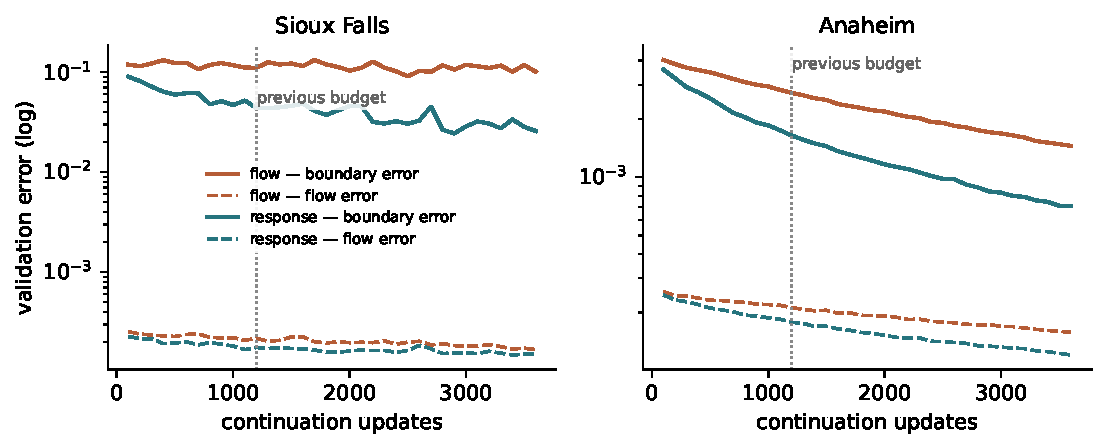
\includegraphics[width=\linewidth]{../figures/fig_v109_convergence.pdf}
\caption{Validation convergence under the extended continuation budget
(seed-median validation boundary error, solid, and relative flow
error, dashed; log scale): Sioux Falls (left) and Anaheim (right),
flow-only (ochre) versus response supervision (teal). The dotted line
marks the 1{,}200-update budget of the main comparison; both
objectives keep improving beyond it, and the response curves stay
below the corresponding flow curves throughout.}\label{fig:v109convergence}
\end{figure}

\subsection{Unrestricted and integrated-bound errors by group}\label{supp:boundchain}
Table~\ref{tab:boundchain96} completes Table~\ref{tab:pathtable} with
the unrestricted and integrated-bound columns of
Eq.~\eqref{eq:localboundarybound}, as percentages of the reference
column's boundary seminorm; the geometric and unrestricted columns use
different denominators and are not one inequality, and the bound chain
$\mathcal K_j(e_j)\le B_j$ holds in absolute units for the shared
quadrature (Section~\ref{sec:pairresults}).
\begin{table}[pos=htbp]\centering\footnotesize
\caption{Unrestricted (exact $\mathcal K_j(e_j)$ over all separating
regions) and bound (integrated bound of
Eq.~\eqref{eq:localboundarybound}) errors, medians of path-level values
on the 96 test paths, as percentages of the reference column's
boundary seminorm.}\label{tab:boundchain96}
\begin{tabular}{rcc cc}\toprule
& \multicolumn{2}{c}{Unrestricted (\%)} & \multicolumn{2}{c}{Bound (\%)}\\
\cmidrule(lr){2-3}\cmidrule(lr){4-5}
Active & flow & resp. & flow & resp.\\\midrule
1 & 4.54 & 2.95 & 4.62 & 3.00\\
2 & 15.48 & 12.65 & 15.67 & 12.80\\
3 & 16.36 & 12.39 & 16.70 & 12.81\\
6 & 19.43 & 12.28 & 20.61 & 13.48\\
\midrule
All 96 & 15.65 & 12.08 & 16.34 & 12.83\\
\bottomrule\end{tabular}\end{table}
